\section{Architecture}
Before diving into the code and its structure, let's take the time to understand how the developers worked. Until \doom, everything was done on a PC. Code was written, compiler generated an executable which ran on the same machine. With the introduction of \NeXT workstations, things had to be different.\\
\par
A developer had two machines, a workstation and PC. All work was done on the \NeXT, code writing, compiling and running using \fixme{Text.app} and \cw{gcc/ld}. Once the developer was happy with the result, he litteraly rolled his chair to the PC where the workstation hard-drive was mounted over NFS. On this side, the PC compiled the same source code\footnote{... with some platform specifics} using Watcom which generated \cw{DOOM.EXE} and ran it. In this setup the PC harddrive was used to boot and host the compiler. Everything else was stored on the \NeXT SCSI HDD.\\
\par
\scaleddrawing{0.9}{dev_setup}{}
\par

There were significant obstacle to sharing the source code. First of all, DOS program had direct access to the hardware whereas NeXT process had to use "official" APIs. Second of all, PC had Intel CPU which are little endian, while Motorola based 68040 were big endian.\\
\par
\pngdrawing{endianness}{}
\par
\ccode{big_little_endian.c}
\par
\ccode{LongSwap.c}
\par
To accomodate the needs of running on different architecture Doom engine is a complete departure from Wolfenstein 3D. The solution they came up with was to have a "kernel" common to all platforms tapping into sub-systems specific to the hardware they supported.\\
\par
\begin{figure}[H]
\centering
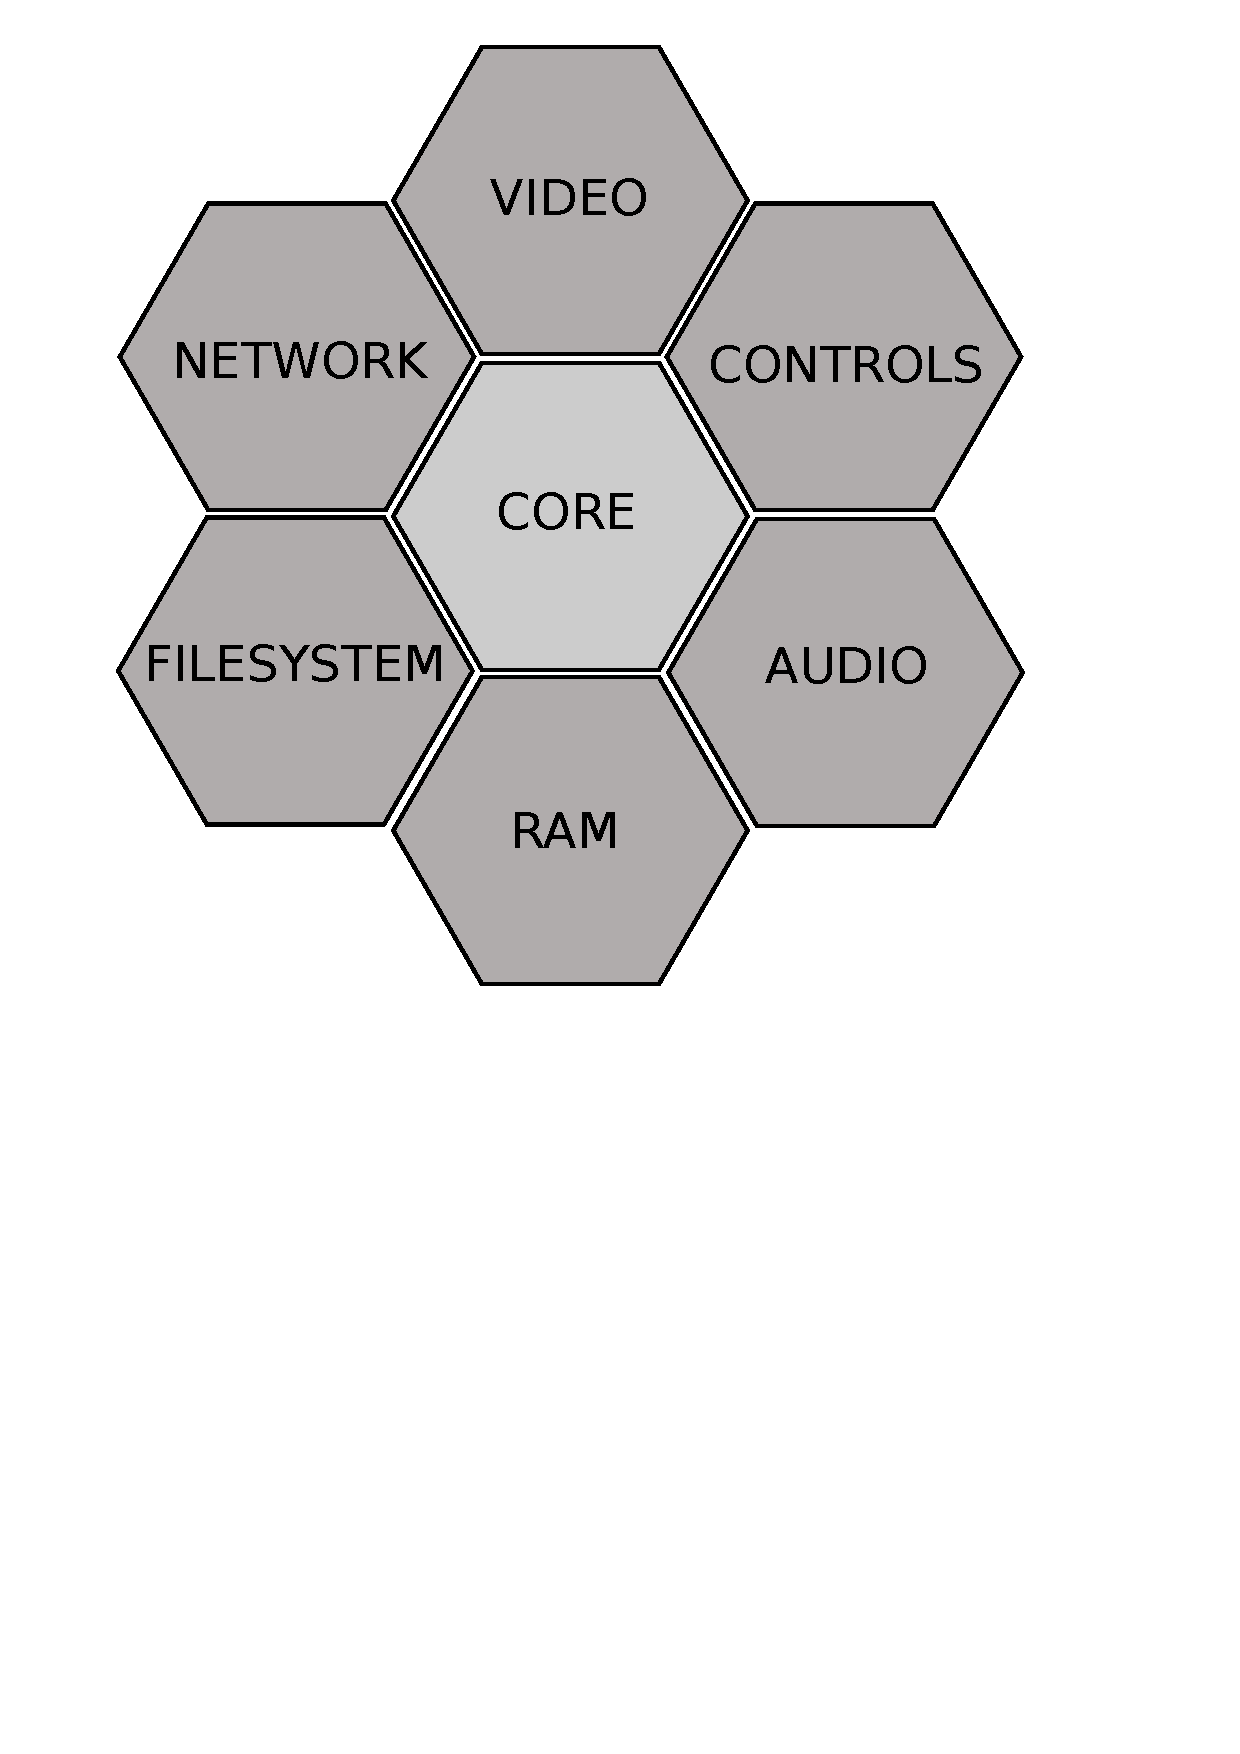
\includegraphics[width=.5\textwidth]{drawings/doom_arch.pdf}
\caption{Doom kernel and its I/O platform-dependent systems.}
\end{figure}
\par
% The kernel six sub-systems are:\\
% \par
% \begin{enumerate}
% \item
% \item
% \item
% \item
% \item
% \item
% \end{enumerate}
The beauty of this system is that once the platform specific system are written, there is zero overheard. All code written runs on both platforms with no modifications.
\par
To implement this system, they exploited the C language ability to declare in a header file (\cw{.h}) a library interface that will only be available later. Each components, the core and all systems for the target plateform are compiled independently during a first step. The C linker combine all object files into an executable (in the case of MS-DOS \cw{DOOM.EXE}).\\
\par
\tcode{s_sound_linker.txt}
\par
Doom ASM improved performances by 16\%. Detail here the method (timedemo) and realtick. FPS 14 to 16.\\
\par


\par

\trivia{
Doom build time\\ 
Full build = 9:37 (among it: 19s to link)\\
Partial build (r\_sky.c) = 27s (among it 19s to link).\\}
\par

Abstraction layer (compare VGA in wolf3d to doom) incured small overhead but also unlocked new algorithm and allowed easy port -> even a fridge runs doom.\\
\par
NextStep dithering.\\
\\ 

\trivia{The MS-DOS source code features what should have been a Doom easter egg. Files \cw{am\_oids.h} and \cw{am\_oids.c} were to allow player to play a remake of Asteroids in the automap but was left unfinished.}\\
\par
\fq{I can’t recall whose idea it was, but it was probably mine.  I was taken by the vector art style of the automap, so Asteroids would have been a good fit, but Doom was behind, and the pace of development at id was incredibly fast.}{Dave Taylor}\\
\par
\tcode{cloc.txt}


\fullimage{Doom_build_NeXTStep.png}
\fakedosoutput{dos_compilation.txt}
\trivia{What are the dot during startup?}

\section{Structure of the code}
The kernel is made of 45 translation units and is common to all version of \doom.\\
\par

\drawing{doom_code_arch}{}
\par

In grey the I/O system which require platform specific code. On DOS six extra files are compiled: \cw{i\_main.c}, \cw{i\_ibm.c}, \cw{planar.asm}, \cw{i\_ibm\_a.asm}, \cw{i\_sound.c} and, \cw{i\_cyber.c}. \\
\par

 \begin{figure}[H]
\centering  
\begin{tabularx}{\textwidth}{ L{0.22} | C{0.39} | C{0.39} }
  \toprule
  \textbf{System} & \textbf{DOS Implementation} & \textbf{NeXT Implementation}\\
  \toprule 
    Video System & VGA & \fixme{X} \\
    Audio System & DMX & Not Implemented\\
    Control System & DMPI Interrupts & \fixme{X} \\
    File  System & Direct & BigEndian converter\\
    Network System & \fixme{X} & \fixme{X} \\
   \toprule
\end{tabularx}
\caption{Platform code specific.}
\end{figure}

\par

\trivia{\NeXT platform specific were all written in Objetive-C: \cw{DRCoord.m}, \cw{VGAView.m}, \cw{Doom\_main.m}, \cw{i\_next.m}, \cw{r\_debug.m},  }

\subsubsection{Hand Optimized Assembler}
There was very little optimized assembler in \doom compared to previous title. The compiler and \cw{libc} were becoming so good that there was no more need to. Only the drawing routines for the walls and flats were optimized wich resulted in a 15\% performance books. \fixme{Graph ASM vs NO ASM}. John Carmack even declared that "The days of assembly are counted". That was without counting on Intel's Pentium which super-scalar architecture would require extra care by Michael Abrash for Quake.
